\section{Theoretical background}
\label{sec:theory}

In this section I will discuss the necessary physical and chemical
background for the construction of the \ch{NO} to \ch{NO2} converter
and the applied measurement methods, which will allow for the
detection of nitrogen oxides ($\ch{NO_x}\ =\ \ch{NO} +
\ch{NO2}$). First, I will describe the chemistry behind the ozone
generator and the influence of ozone on \ch{NO_x}. Next, I will
describe the fluid dynamics of the measurement instrument. After that
I will discuss its influence on the mixing behaviour and the reactions
performed in the converter. Lastly, I will give an introduction to the
differential optical absorption spectroscopy used for the actual trace
gas detection.

\subsection{Ozone chemistry and nitrogen monoxide to nitrogen dioxide conversion}
\label{sec:chemistry}

This section lays the chemical groundwork for the construction of the
\ch{NO} to \ch{NO2} converter. First I will introduce the rate and the
photolysis coefficient to get a measure for the speed of a
reaction. Afterwards I will have a look at possible ways to generate
ozone out of ambient air and then describe ozone induced reactions
concerning nitrogen oxides. This section is mainly inspired by and
taken from~\cite{bsc}.

\subsubsection{The rate and the photolysis coefficient}
\label{sec:rate}

During the conversion there are many chemical reactions of the form

\begin{align}
  \ch{A + B -> C + D}. \label{eq:prototype}
\end{align}

Some of them will have positive effects, others describe side effects
and should be suppressed as much as possible. However, there
are only two parameters to adjust. The first is the ozone
concentration, which can be varied slighty and very roughly, and the
other one is the reaction tube length. Thus the best chance to select
certain reactions is to set their reaction time to a value that
corresponds to the different reaction speeds of the equations, making
sure that desired reactions have enough time to proceed while
simultaneously suppressing unwanted reactions. Of course this is only
possible, if the desired reactions run faster than the unwanted ones.

With this motivation in mind, I would like to introduce a measure for
the reaction speed. Thinking of speed in this setting means to think
of the change of compound concentration. In this section I will use
$c$ (in \si{\per\cubic\centi\meter}) to denote concentrations. Using
the above mentioned prototypic equation, one can see that the change
of concentration, i.\,e. $\dot c$, of the different species are
related by:
\begin{align*}
  -\dot c(A) = - \dot c(B) = \dot c(C) = \dot c(D).
\end{align*}
Naturally, this is only true, if Reaction~\eqref{eq:prototype} is the
only reaction concerned with the above mentioned species.

Next I need a relation between these derivatives and the educt
concentrations. The probability for a reaction to take place should be
proportional to both to $c(A)$ and $c(B)$ as the two molecules need to
`meet'. Thus it seems plausible to expect
\begin{align}
  -\dot c(A) = - \dot c(B) = k \cdot c(A) \cdot c(B), \label{eq:rate}
\end{align}
where the proportionality constant $k$ ist called \emph{rate
  coefficient}. It is often given in units of
\si{\hertz\cubic\centi\meter}. This $k$ is the desired reaction
speed measure, as it describes the
reaction time independently of the compound concentrations.

In the case of the conversion, the ozone concentration will far exceed
the concentration of the other trace gases. This allows one to think
of its concentration as approximately constant. If $c(B)$ is set
constant in Equation~\eqref{eq:rate}, then this yields a well known
ordinary first order differential equation for $c(A)$ with the
solution
\begin{align*}
  c(A,t) = c(A,0)\exp(-kc(B)\cdot t).
\end{align*}
In this limiting case one sees that the reaction time is given by $\tau =
(kc(B))^{-1}$, making the connection of $k$ to the reaction speed
obvious.

There is a second important reaction type for this work:
\emph{photolysis} reactions. These take the form

\begin{align}
  \ch{A + h}\nu \ch{-> C + D},
\end{align}
i.\,e.\ one of the educts is replaced by a photon. In this case, the
differential equation connecting the concentration is
\begin{align}
  \dot c(C) = \dot c(D) = -\dot c(A) = - j(\nu) \cdot c(A),
\end{align}
where the wavelength dependence of the reaction speed has been
transferred to the \emph{photolysis coefficient} $j(\nu)$. As before,
this equation only holds, if there are no other reactions taking place
simultaneously. Since $j$ has a rather complex wavelength and
intensity dependence, it is difficult to give a closed formula, making
it impossible to simply give a fixed value in the reaction
equations. Therefore, the exact value will be omitted in all photolysis
equations and instead the wavelength limit for an ignition if the
reaction will be stated.

\subsubsection{Ozone generation}
\label{sec:theory-ozone}

In this section I will discuss the generation of ozone (\ch{O3}) out of ambient
air. The main idea comes from the observation that stratospheric
\ch{O3} protects us from ultraviolet (UV) light. Thus ozone needs to
have absorption bands there. Furthermore, normally, the ozone layer is
not depleted, but regenerates itself, so one can suspect a reaction
cycle building ozone out of ordinary oxygen molecules (\ch{O2}).

The following equations describe the ozone-oxygen cycle in the
atmosphere.  It is often referred to as \emph{Chapman-Cycle} due to
its first investigator (c.\,f.~\cite{chapman,roedel}). As it turns
out, one can use these atmospheric reactions to generate ozone in the
laboratory.

In some of the reactions an additional molecule is necessary to assure
momentum conservation. This inert reaction participant is always
denoted \ch{M}. The first part of the cycle contains the reactions,
that generate \ch{O3} out of \ch{O2}

\begin{align}
  \ch{O2 + h}\nu &\ch{->[\phantom{$k=\SI{5.6e-34}{\hertz\cubic\centi\meter}$}] 2 O(^3P)},\nonumber\\
  \ch{O(^3 P) + O2 + M} &\ch{->[$k=\SI{5.6e-34}{\hertz\cubic\centi\meter}$] O3 + M}. \label{eq:ozone}
\end{align}
A photon splits an oxygen molecule and the excited oxygen atom reacts
with another \ch{O2} molecule to form ozone. For the first reaction to
take place a photon of the wavelength
$\lambda < \SI{240}{\nano\meter}$ is necessary.

The next part of the cycle shows, how another UV photon ($\lambda <
\SI{310}{\nano\meter}$) can destroy
ozone and create a ground state oxygen atom. This oxygen atom will
then be reexcited:

\begin{align}
  \ch{O3 + h}\nu \ch{&->[\phantom{$k=\SI{2.6e-11}{\hertz\cubic\centi\meter}$}] O(^1 D) +
  O2}, \label{eq:split}\\
  \ch{O(^1 D) + M & ->[$k=\SI{2.6e-11}{\hertz\cubic\centi\meter}$] O(^3 P) + M}.\nonumber
\end{align}
After this reaction there are two possible reaction paths. First the $\ch{O}(^3
P)$ can reenter Reaction~\eqref{eq:ozone}, such that there is no
net change in ozone or it can react to form \ch{O2} by the
following mechanism

\begin{align*}
  \ch{O(^3 P) + O3 & ->[$k=\SI{8.0e-15}{\hertz\cubic\centi\meter}$] 2 O2},
\end{align*}
leading to a net loss of ozone. 

Introducing a UV light source with an emission below
$\lambda < \SI{240}{\nano\meter}$ will start the above cycle. In this
case a mercury lamp is used, which also has a strong peak at
$\lambda = \SI{254}{\nano\meter}$. So the Chapman-Cycle will enter an
equilibrium state with a constant ozone oxygen ratio. The value of
this ratio depends on the intensity ratio at the two wavelength ranges
of the above mentioned photolysis reactions. Since the main energy
output of the lamp is at \SI{254}{\nano\meter}, the ratio will be
small. However, there is around \SI{20}{\%} oxygen in ambient air,
such that in absolute terms there will still be a considerable surplus
of ozone. The expected ozone value can be computed exactly using the
photolysis coefficients of the reactions and this has been done
in~\cite{bsc}. Using this specific lamp leads to a value of
$c(\ch{O3}) = \SI{300}{ppm}$. Of course this value will vary for
different electric currents at the lamp, but since the exact value is
of no special interest, a magnitude suffices. This estimate will be
enough for this purpose. The experimentally verified output of the
built generator can be found in Section~\ref{sec:ozone}.

\subsubsection{Ozone triggerd nitrogen oxide reactions}
\label{sec:o-no}

In this section I will have a look at all reactions concerning
chemicals consisting of nitrogen and oxygen. The aim is to achieve a
complete conversion of nitrogen monoxide (\ch{NO}, also referred to as
nitric oxide) to nitrogen dioxide (\ch{NO2}). However, introducing
ozone to the sample air triggers further reactions. If these lead to a
net change of \ch{NO2} there are additional effects to correct. All
reactions are given with their corresponding rate coefficient $k$
which were taken from~\cite{bsc}. In Section~\ref{sec:requirements} I
will discuss the implications of the reactions here on the setup of
the converter.

The desired reaction is the following

\begin{align}
  \ch{NO + O3 & ->[$k=\SI{1.8e-14}{\hertz\cubic\centi\meter}$] NO2
                + O2}. \label{eq:no}
\end{align}
If this were the only reaction, there would be a one to one conversion
from \ch{NO} to \ch{NO2}. With enough ozone the goal of the converter
would be achieved. However, this is not the case. Nitrogen dioxide
itself can be oxidized by ozone to generate nitrogen trioxide
(\ch{NO3}):

\begin{align}
  \ch{NO2 + O3 ->[$k=\SI{3.5e-17}{\hertz\cubic\centi\meter}$] NO3
  + O2}. \label{eq:no2}
\end{align}
Luckily, the rate coefficients of the two reactions are very different
and the first one is approximately three orders of magnitude larger
than the second one.

Additionally there is a very fast reaction of \ch{NO3} with \ch{NO}
\begin{align}
  \ch{NO + NO3 ->[$k=\SI{6.9e-2}{\hertz\cubic\centi\meter}$] 2 NO2},\label{eq:back}
\end{align}
such that small nitrogen trioxide concentrations should decay
quickly. If one assumes no \ch{NO3} in the sample air (which is sensible
for day time measurements) Equation~\eqref{eq:back} should guarantee
that the oxidation of \ch{NO2} should be compensated. 

Sadly, this is not the only reaction using \ch{NO3}. It can react
with \ch{NO2} to generate the solid \ch{N2O5}

\begin{align}
  \ch{NO2 + NO3 + M
  <=>[$k=\SI{1.9e-12}{\hertz\cubic\centi\meter}$][$k=\SI{2.6e-11}{\hertz\cubic\centi\meter}$]
  N2O5 + M}. \label{eq:laughing}
\end{align}
As the rate coefficients show, the equilibrium of
Equation~\eqref{eq:laughing} lies on the side of the educts, such that
the effect should not be too large. Especially if the \ch{NO3}
concentrations are small. In the further analysis I will assume that
the reaction time is set in such a way that Equation~\eqref{eq:no}
can proceed while Equation~\eqref{eq:no2} is still suppressed. This
will make it possible to simply ignore the reaction paths for \ch{NO3}.

There is yet another reaction cycle going on in the ozone
generator. This one is concerned with nitrous oxide (\ch{N2O}) also
known as laughing gas. It has a strong absorption cross section in the
range of \num{185} to \SI{230}{\nano\meter}, which triggers the
following dissociation reaction
\begin{align}
  \ch{N2O + h}\nu \ch{->[\phantom{$k=\SI{7.2e-11}{\hertz\cubic\centi\meter}$}] N2 + O(^1 D)}.\label{eq:n2o-good}
\end{align}
This reaction in itself is not very interesting in this setting, as
neither nitrogen nor oxygen interfere with the measurements. However
there are other reaction pathways by which \ch{N2O} can degrade and
these need the excited $\ch{O(^1D)}$ atom, which can come either from
Equation~\eqref{eq:ozone} or~\eqref{eq:n2o-good}. In this case the two
other possible reactions are
\begin{align}
  \ch{N2O + O(^1 D) & ->[$k=\SI{7.2e-11}{\hertz\cubic\centi\meter}$] 2 NO} \qquad \text{and}\label{eq:n2o-bad}\\
  \ch{N2O + O(^1 D) & ->[$k=\SI{4.4e-11}{\hertz\cubic\centi\meter}$] N2 + O2}, \nonumber
\end{align}
where the first path is slightly favored (c.\,f.~\cite{n2o}). All in
all most of the laughing gas should degrade over the photolysis in
Reaction~\eqref{eq:n2o-good}, as the lamp has lines in this range.
However, since the ozone generator produces quite a high amount of
excited oxygen atoms, the other pathways, with
Reaction~\eqref{eq:n2o-bad} being especially worrisome, cannot be
ignored. Additional nitrogen monoxide will lead to additional nitrogen
dioxide, which will in turn will istort the measurement results. As
will be seen in Section~\ref{sec:adsorption}, this problem cannot be
solved by filtering \ch{N2O} as it passes most barriers, so the
reaction products have to be removed after the transition took place.

\subsection{Basics of fluid dynamics}
\label{sec:fluid}

One important aspect of this work consists in the understanding of the
different gas flows in the instrument. I need an estimate for the
mixing time of ozone with the sample air in order to be able to choose
the correct reaction tube length. Only then can a full conversion be
achieved. This problem can be solved using a few basic principles from
fluid dynamics. First, I will have a look at laminar flows in
cylindric vessels (in this case tubes) to get a connection between the
flow and the maximum speed in the tube. Next I will have a look at
diffusion of gases. As there will only be laminar flows, diffusion is
the only way mixing can take place, so an estimate for the mixing time
due to diffusion is required. Lastly, I will discuss adsorption of
trace gases at teflon, silica gel and activated carbon as this is an
important property of the instrument.

\subsubsection{Laminar flows in cylinders}
\label{sec:cylinder}

It is important to know in what regime the gas transport in the tube
settles. Especially after the ozone enriched air is added to the
sample air, it would be beneficial to have a turbulent flow in the
system as it would ensure a faster mixing of the gases. In order to see whether
one can expect a laminar or a turbulent flow, the phenomenological
\emph{Reynold's number} is used,

\begin{align*}
  \operatorname{Re} = \frac{\rho \cdot d \cdot \bar v}{\eta},
\end{align*}
where $\rho$ denotes the density of the gas, $d$ is a characteristc
length of the system, in this case the tube diameter, $\bar v$ is the
average velocity of the gas and $\eta$ its viscosity. As a rule of
thumb the flow in a cylinder will be laminar, if the Reynold's number
is smaller than the critical Reynold's number
$\operatorname{Re}_{\text{c}} = 2300$ and it will be turbulent if the
number is higher than $3000$ (c.\,f.~\cite{maschbau}). In this system
this means $d = \SI{4}{\milli\meter}$,
$\rho \approx \SI{1.2}{\kilo\gram\cubic\meter}$ and
$\eta \approx \SI{17.1}{\micro\pascal\second}$
(c.\,f.~\cite{maschbau}). Furthermore, the cavity operates at a flow
of $\Phi = \SI{2}{\liter\per\minute}$. With the above diameter this
leads to an average velocity of
$\bar v = \SI{2.7}{\meter\per\second}$. Using this data the Reynold's
number is computed to be

\begin{align*}
  \operatorname{Re} \approx 760 < 2300.
\end{align*}
Thus one can expect to work solely in the laminar regime and a good
understanding of the velocity distribution in this case is needed in
order to allow enough time for mixing and the chemical reactions to
take place. The law behind the laminar flow in a cylindric tube is
called \emph{Hagen-Poiseulle} and I will follow the exposition used
in~\cite{gerthsen} to derive it.

Denote by $r_0$ the inner radius of the tube and by $l$ its
length. Let furthermore the gas flow be in an equilibrium state, such
that all forces need to add to zero. Consider a gas <cylinder of radius
$0 \leq r \leq r_0$. In order to have a nonzero flow, there needs to be a
pressure difference at the two ends of the tube denoted by $\Delta
p$. The force exerted on the cylinder by the pressure is given by
\begin{align*}
  F_b = - \pi r^2 \Delta p,
\end{align*}
where the minus sign is introduced because the force points in the
opposite direction of the pressure gradient. At the boundary of the
cylinder there is friction between the adjoining layers of fluid. The
force exerted by it is proportional to the area of friction, i.\,e.\
the cylinder barrel, and to the difference in velocity between the
fluid within the cylinder and outside. Since this means talking about
the velocity difference on an infinitesimal anulus around the
boundary, this leads to a proportionality to the velocity gradient
$\frac{\d[v]}{\d[r]}$. Thus the force of friction takes the form

\begin{align*}
  F_f = \eta \cdot 2\pi r \cdot l \cdot \frac{\d[v]}{\d[r]},
\end{align*}
where $\eta$ is again the viscosity of the gas. The fluid is assumed
to be in an equilibrium, thus $F_b = F_f$ needs to hold for all
possible $r$. This leads to the following differential equation for
the velocity

\begin{align*}
  \frac{\d[v]}{\d[r]} = - \frac{\Delta p}{2l\eta} \cdot r
\end{align*}
which can be integrated. Using the boundary condition $v(r_0)
= 0$, i.\,e.\ the fluid sticks to the wall of the tube, one gets

\begin{align}
  v(r) = v_0 \left ( 1 - \left( \frac{r}{r_0} \right)^2 \right) \quad
  \text{with }\ v_0 \coloneqq \frac{\Delta p r_0^2}{4 l \eta}. \label{eq:v}
\end{align}
This can be further integrated to yield the flow $\Phi$ of the system

\begin{align*}
  \Phi = \int_A v(r) \d[A] = 2\pi \int_0^{r_0} v(r)r \d[r] = \frac{\pi
  r_0^4}{8\eta l} \cdot \Delta p.
\end{align*}
This is the standard form of the Hagen-Poiseulle law. One remarkable
observation is that there is a power four law between the radius of
the tube and the flow. More interesting for this work is the relation
between the average velocity $\bar v$ and the maximum velocity $v_0$
at the center of the pipe

\begin{align*}
  \bar v = \frac{\Phi}{\pi r_0^2} = \frac{\Delta p r_0^2}{8\eta l} \stackrel{\eqref{eq:v}}{=} \frac{v_0}{2},
\end{align*}
i.\,e.\ at the center the velocity is twice as large as the
average. This effect should be kept in mind when it comes to the
computation of the dwell time of the gases.

\subsubsection{Diffusion}
\label{sec:diffusion}

As was shown in the previous section, the gas flows laminarly
throughout the instrument. Thus the only mechanism by which gas mixing
can occur is \emph{diffusion}. Therefore I would like to get an
estimate for the time it takes for diffusion to take place. This
exposition drew inspiration from~\cite{fluid}.

In order to understand diffusion of a species, one has to investigate
the evolution of its concentration $n$ (in \SI{1}{\per\cubic\meter}).
Fick's first law states that the particle current density $j$ (in
\SI{1}{\per\square\meter\second}) of the species is proportional to
the concentration gradient $\nabla n$ and that the species flows from
higher to lower concentrations. This leads to

\begin{align*}
  j = - D \nabla n,
\end{align*}
where $D > 0$ (in \SI{1}{\square\meter\per\second}) is called the
\emph{diffusion constant}. Assuming no sources and sinks and using the
continuity equation for fluids, one arrives at Fick's second law

\begin{align*}
  \dot n = - \nabla j = \nabla (D \nabla n) = D \cdot \Delta n,
\end{align*}
where for the last equation an isotrope medium, i.\,e.\
$\nabla D = 0$, was assumed. This is a second order linear partial
differential equation and for arbitrary boundary conditions it can
become arbitrarily hard to solve. Since in this work's setup diffusion
of species at small time scales is of interest, the vessel can be
assumed inifinitely large. With this the equation becomes accessible
via Fourier analysis. Let

\begin{align*}
  \hat n(k,t) = \mathcal{F}[n](k,t)
\end{align*}
be the Fourier transform of $n$ with regard to the three spatial
coordinates $x$. Using the known relation $\mathcal{F}[\partial_{x_j}
n](k,t) = -ik_j \hat n(k,t)$, one can transform the equation to

\begin{align*}
  \partial_t \hat n(k,t) =  - D|k|^2 \hat n(k,t)
\end{align*}
which is a linar first order ordinary differential equation, with the
well known solution

\begin{align}
  \hat n(k,t) = c(k) \cdot \exp(-D|k|^2 t). \label{eq:sol-ft}
\end{align}
In order to determine $c(k)$, an initial value is required. Again an
idealistic, simplified model is applied. I will later on be interested
in the diffusion of one molecule. Therefore, the initial condition
\begin{align*}
  n(x,0) = n_0 \delta(x)
\end{align*}
is chosen, i.\,e.\ all the species (or for $n_0 = 1$: the particle) is
localized at one point for $t = 0$. One can Fourier transform this
initial condition, too, and yield

\begin{align*}
  \hat n(k,0) = n_0.
\end{align*}
Plugging this into Equation~\eqref{eq:sol-ft}, leads to

\begin{align*}
  \hat n(k,t) = n_0 \exp(-Dt \cdot |k|^2).
\end{align*}
This is a Gaußian function with regard to the variable $k$. In order
to get the solution of the diffusion equation in terms of $x$ the
computation of the inverse Fourier transform of $\hat n$ has to be
performed. However, it is a well known fact that the Gauß function is
an Eigenfunction of the Fourier transform (and its
inverse). Additionally the total concentration needs to be constant
for all times $t$, which gives its normalization. Thus the solution
has to take the form

\begin{align*}
  n(x,t) = \frac{n_0}{(2\pi \cdot 2Dt)^{3/2}} \cdot \exp \left(
  -\frac{1}{2} \cdot \frac{|x|^2}{2Dt} \right).
\end{align*}
This makes it possible to describe the statistical behaviour of a particle
undergoing diffusion. Setting $n_0 = 1$ leads to the probability
distribution for the particle, which is just a Gaußian distribution
with a timedependent variance. The expectation value of
the position $\langle x \rangle$ is always 0. However the standard
deviation $\sigma = \sqrt{2Dt}$ grows larger over time, such that for
the \emph{mean squared displacement}, one gets the following relation

\begin{align}
  \langle |x|^2 \rangle = \sum_{j=1}^3 \langle
  x_j^2 \rangle = \sum_{j=1}^3 \sigma^2 = 3 \cdot 2Dt, \label{eq:mqd}
\end{align}

where $\langle x \rangle = 0$ was needed. This mean squared
displacement can now be used as a measure to gauge the distance
travelled by a molecule. I will apply it to gauge the time needed for
a new gas species (in this case ozone) to fill a volume sufficiently
for the chemical reactions to take place.

\subsubsection{Adsorption}
\label{sec:adsorption}

Adsorption plays an important role in the setup of the instrument. The
zero air has to be free of all trace gases to be measured. Experience
shows that a filter chain of activated carbon, silica gel and a
particle filter is sufficient for this process. One would assume that
this air stream is also sufficiently pure to be used in the ozone
generator. Sadly, this is not true as was for example noted
in~\cite{bsc}.

After the air passes the generator there is a \ch{NO2} signal in the
range of \num{1} to \SI{10}{ppb}, which is well detectable by CE-DOAS
instruments. The cause was found to be laughing gas, which is a
normally inert and badly soluble gas. Therefore, it passes all used
filters in high enough concentrations such that
Reaction~\eqref{eq:n2o-bad} has to be taken into account. The produced
\ch{NO} then leads to the perceived \ch{NO2} signal.

As filtering of the laughing gas in front of the generator could not
be achieved, the possibilty of filtering the nitrogen dioxide after
the ozone generator are explored here. This poses the difficulty of
filtering it without removing the ozone, too. Rubin~\cite{ozone-silica}
mentions that silica gel can be used as an ozone storage
device, but with a limited capacity. Furthermore, it is known that
silica is a good \ch{NO2} filter due to its good solubility in
water. Hence the idea to use silica gel. At first it will be
impenetrable by the ozone as well as by the nitrogen dioxide, but as
soon as the ozone saturation level is reached, it will pass, while the
\ch{NO2} is still kept back. The experimental viability of this idea
was tested in Sections~\ref{sec:ozone} and~\ref{sec:silica}.

Another effect one has to consider is the adsorption of the gases at
the teflon walls of the tube. Experience from previous setups shows
that this effect is rather small. The influence on the sample air is a
systematic uncertainty in any case and has to be considered for any
CE-DOAS measurement, so the only question remaining is, whether the
adsorption has an impact on the ozone flow. As in this setting there
are rather large concentrations in the order of magnitude of \si{ppm},
I suspect this not to be the case after an equilibrium has been
reached. The \ch{NO} concentration is normally on the order of
magnitude of a few \SI{10}{ppb} or perhaps a few \SI{100}{ppb} if one
considers downtown stationary measurements. So for all reasonable
adsorption capacities there is always enough ozone left for the full
conversion. The only interesting instance is during a switch where the
ozone stream is turned off to only measure \ch{NO2}. Here the
evaporation of ozone could lead to longer purge times and hence to a
worse time resolution. The behaviour of the system after such switches
has been researched in Section~\ref{sec:switch}.

\subsection{Technical requirements for the converter}
\label{sec:requirements}

The above considerations lead to some technical requirements in the
construction of the converter. First and obviously well filtered air
in the ozone generator is obligatory in order to avoid additional
trace gas contamination which would disturb the measurement. The
normal procedure consists of using an activated carbon, a silica gel
and a particle filter. In order to compensate for the laughing gas mentioned in
Section~\ref{sec:adsorption}, a silica gel filter after the ozone
generator is introduced. For the filtering to be effective, some tube
length has to be added between the ozone generation chamber and the
silica gel filter, such that the conversion from \ch{N2O} to \ch{NO2}
can be completed.

The next restriction is that a nigh \SI{100}{\%} conversion of \ch{NO}
to \ch{NO2} is necessary. This leads to three considerations. Firstly,
there needs to be enough time for the mixing of the ozone with the
sample air to take place. Secondly, there needs to be enough time for
the actual reaction to take place. Thirdly, there must not be the time 
for considerable losses in \ch{NO2} due to further oxidation.

Concering the mixing with ozone, Section~\ref{sec:fluid} supplies an
estimate of the mixing time. As there are mainly laminar flows in the
reaction path (c.\,f.\ Sec.~\ref{sec:cylinder}), the mixing will be
dominated by diffusion. Thus the mean squared displacement is used to
estimate the time the ozone takes to cross the tube diameter. In this
case tubes with $d = \SI{4}{\milli\meter}$ are used and the diffusion
constant for ozone in air was taken to be
$D = \SI{0.137}{\square\centi\meter\per\second}$ (at
$T = \SI{298}{\kelvin}$ and $p = \SI{1}{\text{bar}}$
c.\,f.~\cite{diff-ozone}). This leads to
\begin{align*}
  t_{\text{mix}} \approx \frac{d^2}{6\cdot D} = \SI{0.195}{\second}
\end{align*}

Turning towards considerations two and three, the reaction time has to
be adjusted. For this the desired conversion ratio was set to
\SI{99}{\%}. Since the ozone generator will supply an overabundance of
\ch{O3}, the linear ordinary differential equation approximation
introduced in Section~\ref{sec:rate} is applicable. Thus the
conversion ratio is given by
\begin{align*}
  \exp(-kc(\ch{O3})\cdot t),
\end{align*}
where $t$ is the reaction time. $1$ stands for no
conversion at all (i.\,e.\ no decrease in the educt concentration) and
$0$ stands for complete conversion. In order to get \SI{99}{\%} for
the exponent the following condition needs to hold
\begin{align}
  kc(\ch{O3}) \cdot t_{\text{react}} \gtrsim 4.6. \label{eq:react-bound}
\end{align}
As a lower bound for the ozone concentration 
\begin{align*}
  c(\ch{O3}) = \SI{2}{ppm} = \SI{4.996e13}{\per\cubic\centi\meter} 
\end{align*}
is chosen and using $k = \SI{1.8e-14}{\hertz\per\cubic\centi\meter}$,
leads to the following natural time scale
\begin{align*}
  \tau^{-1} & = k c(\ch{O3}) = \SI{0.90}{\per\second}.
\end{align*}
Together with Equation~\eqref{eq:react-bound} this yields
\begin{align*}
  t_{\text{react}} \gtrsim \SI{5.1}{\second}.
\end{align*}
Using $t_{\text{react}}$ to compute the conversion ratio of $\ch{NO2}$
to $\ch{NO3}$, the result is \SI{0.9}{\%}. So with this reaction time
one should expect about a \SI{2}{\%} error in the retrieved \ch{NO}
concentration. Hopefully, the results will be better than that, as
some of the produced \ch{NO3} will (as described in
Section~\ref{sec:o-no}) quickly degrade to \ch{NO2} and the ozone
concentration is likely to be underestimated.

As a last step I would like to translate the needed mixing and reaction
time
\begin{align*}
  t = t_{\text{mix}} + t_{\text{react}} = \SI{5.3}{\second}
\end{align*}
to its associated tube length. Using the applied flow of
$\Phi = \SI{2}{\liter\per\minute}$, the average velocity of the gas
can be computed to be
\begin{align*}
  \bar v = \frac{\Phi}{\pi r^2} = \SI{2.7}{\meter\per\second}. 
\end{align*}
As was described in Section~\ref{sec:cylinder} this corresponds to a
maximum velocity at the center of the tube of

\begin{align*}
  v_0 = 2\cdot \bar v = \SI{5.4}{\meter\per\second}.
\end{align*}
Using these two velocities leads to

\begin{align*}
  \bar l & = \SI{14.31}{\meter} \quad \text{and}\\
  l_0 & = \SI{28.62}{\meter}
\end{align*}
as tube lengths.

For the experiment the used tube length was geared to $\bar l$, as the
maximum velocity is only relevant for a rather small cross section of
the cylinder. Most experiments were performed at
$l = \SI{10}{\meter}$, such that part of the conversion reaction was
taking place inside the cavity. The idea behind this is to have the
conversion peak close to the center of the cavity as this should lead
to the best conversion ratio averaged over all the cavity.

\subsection{The physics behind CE-DOAS}
\label{sec:ce-doas-physics}

In the following sections I will discuss the physical concepts
necessary to understand the \emph{Cavity Enhanced Diffirential
  Absorption Spectroscopy} (CE-DOAS). First, I will investigate the
Lambert-Beer Law. This leads directly to the so called
\emph{Longpath}-DOAS instrument. As the name already indicates, those
need a long lightpath, since often the absorption cross sections of
the investigated trace gases are very small. Hence, lastly, the
\emph{cavity enhancement} is introduced to overcome this restriction.

The presentation follows mostly~\cite{fp58} with a few inspirations
taken from~\cite{bsc} and~\cite{platt}.

\subsubsection{The Lambert-Beer Law}
\label{sec:lambert-beer}

The \emph{Lambert-Beer Law} ist the underlying principle behind the
main measurement method used in this work. It concerns itself with the
evolution of the light intensity $I_0$ which propagates a certain
distance $L$ through air (or other absorbing matter). It assumes an
exponential decay over $L$, so one can write

\begin{align}
  I(\lambda, L) = I_0(\lambda) \cdot \exp[-\epsilon(\lambda) \cdot
  L], \label{eq:lb-easy}
\end{align}
where $\epsilon$ is called the \emph{absorption coefficient}. This
coefficient contains all the influences of the matter on the
absorption behaviour and can thus be split to account for the different
absorption and scattering mechanisms:

\begin{align*}
  \epsilon = \epsilon_a + \epsilon_R + \epsilon_M,
\end{align*}
where $\epsilon_a$ denotes the absorption and scattering due to the
trace gases, $\epsilon_R$ denotes Rayleigh scattering and $\epsilon_M$
Mie scattering. Next, a better understanding of the relationship
between the trace gases and $\epsilon_a$ is necessary. The absorption
should be proportional to the concentration of the gases, so one
writes

\begin{align}
  \epsilon_a(\lambda) = \sum_{i=1}^n \sigma_i(\lambda) \cdot \bar c_i, \label{eq:lb-abs}
\end{align}
where $i$ sums over all the trace gases present in the penetrated air,
$\bar c_i$ is the associated average concentration and $\sigma_i$ is
calld \emph{absorption cross section}. For the above formula to be
useful to determine the concentration of the trace gases, a very
homogenous air sample is required, so that the average concentration
is meaningful. As will be seen, this assumption is sensible for
CE-DOAS, if one works with Longpath-DOAS measurements one has to work
with other parameters, e.\,g.\ the collumn density.

Equations~\eqref{eq:lb-easy} and~\eqref{eq:lb-abs} now contain the
central idea for the spectroscopic method. One can measure the
intensity spectra $I$ and $I_0$, one can also determine the pathlength
$L$. If one next wants to compute the concentration of the trace gases,
only the absorption cross sections are required, which can be found in the
literature. Thus lastly the \emph{Optical Density} is introduced

\begin{align*}
  D(\lambda) = \ln \left(\frac{I(\lambda)}{I_0(\lambda)}\right) = - L
  \cdot \sum_{i=1}^n \sigma_i(\lambda) c_i,
\end{align*}
containing all the necessary information for trace gas measurements.

\subsubsection{The DOAS method}
\label{sec:doas}

\emph{Differential Optical Absorption Spectroscopy} uses the
Lambert-Beer Law to compute the concentrations of trace gases in the
air. There are a few more technicalities to be taken care of. First of
all, an analysis of the absorption cross sections of different trace
gases has to be done. If they are meant to distinguish different gases
and even compute their concentration, they need to be sufficiently
separating.

\begin{figure}[htbp]
  \centering
  % GNUPLOT: LaTeX picture with Postscript
\begingroup
  \makeatletter
  \providecommand\color[2][]{%
    \GenericError{(gnuplot) \space\space\space\@spaces}{%
      Package color not loaded in conjunction with
      terminal option `colourtext'%
    }{See the gnuplot documentation for explanation.%
    }{Either use 'blacktext' in gnuplot or load the package
      color.sty in LaTeX.}%
    \renewcommand\color[2][]{}%
  }%
  \providecommand\includegraphics[2][]{%
    \GenericError{(gnuplot) \space\space\space\@spaces}{%
      Package graphicx or graphics not loaded%
    }{See the gnuplot documentation for explanation.%
    }{The gnuplot epslatex terminal needs graphicx.sty or graphics.sty.}%
    \renewcommand\includegraphics[2][]{}%
  }%
  \providecommand\rotatebox[2]{#2}%
  \@ifundefined{ifGPcolor}{%
    \newif\ifGPcolor
    \GPcolorfalse
  }{}%
  \@ifundefined{ifGPblacktext}{%
    \newif\ifGPblacktext
    \GPblacktexttrue
  }{}%
  % define a \g@addto@macro without @ in the name:
  \let\gplgaddtomacro\g@addto@macro
  % define empty templates for all commands taking text:
  \gdef\gplbacktext{}%
  \gdef\gplfronttext{}%
  \makeatother
  \ifGPblacktext
    % no textcolor at all
    \def\colorrgb#1{}%
    \def\colorgray#1{}%
  \else
    % gray or color?
    \ifGPcolor
      \def\colorrgb#1{\color[rgb]{#1}}%
      \def\colorgray#1{\color[gray]{#1}}%
      \expandafter\def\csname LTw\endcsname{\color{white}}%
      \expandafter\def\csname LTb\endcsname{\color{black}}%
      \expandafter\def\csname LTa\endcsname{\color{black}}%
      \expandafter\def\csname LT0\endcsname{\color[rgb]{1,0,0}}%
      \expandafter\def\csname LT1\endcsname{\color[rgb]{0,1,0}}%
      \expandafter\def\csname LT2\endcsname{\color[rgb]{0,0,1}}%
      \expandafter\def\csname LT3\endcsname{\color[rgb]{1,0,1}}%
      \expandafter\def\csname LT4\endcsname{\color[rgb]{0,1,1}}%
      \expandafter\def\csname LT5\endcsname{\color[rgb]{1,1,0}}%
      \expandafter\def\csname LT6\endcsname{\color[rgb]{0,0,0}}%
      \expandafter\def\csname LT7\endcsname{\color[rgb]{1,0.3,0}}%
      \expandafter\def\csname LT8\endcsname{\color[rgb]{0.5,0.5,0.5}}%
    \else
      % gray
      \def\colorrgb#1{\color{black}}%
      \def\colorgray#1{\color[gray]{#1}}%
      \expandafter\def\csname LTw\endcsname{\color{white}}%
      \expandafter\def\csname LTb\endcsname{\color{black}}%
      \expandafter\def\csname LTa\endcsname{\color{black}}%
      \expandafter\def\csname LT0\endcsname{\color{black}}%
      \expandafter\def\csname LT1\endcsname{\color{black}}%
      \expandafter\def\csname LT2\endcsname{\color{black}}%
      \expandafter\def\csname LT3\endcsname{\color{black}}%
      \expandafter\def\csname LT4\endcsname{\color{black}}%
      \expandafter\def\csname LT5\endcsname{\color{black}}%
      \expandafter\def\csname LT6\endcsname{\color{black}}%
      \expandafter\def\csname LT7\endcsname{\color{black}}%
      \expandafter\def\csname LT8\endcsname{\color{black}}%
    \fi
  \fi
    \setlength{\unitlength}{0.0500bp}%
    \ifx\gptboxheight\undefined%
      \newlength{\gptboxheight}%
      \newlength{\gptboxwidth}%
      \newsavebox{\gptboxtext}%
    \fi%
    \setlength{\fboxrule}{0.5pt}%
    \setlength{\fboxsep}{1pt}%
\begin{picture}(8062.00,10080.00)%
      \csname LTb\endcsname%
      \put(4031,9860){\makebox(0,0){\strut{}}}%
    \gplgaddtomacro\gplbacktext{%
      \csname LTb\endcsname%
      \put(550,7013){\makebox(0,0)[r]{\strut{}$2$}}%
      \put(550,7443){\makebox(0,0)[r]{\strut{}$3$}}%
      \put(550,7874){\makebox(0,0)[r]{\strut{}$4$}}%
      \put(550,8304){\makebox(0,0)[r]{\strut{}$5$}}%
      \put(550,8734){\makebox(0,0)[r]{\strut{}$6$}}%
      \put(550,9165){\makebox(0,0)[r]{\strut{}$7$}}%
      \put(550,9595){\makebox(0,0)[r]{\strut{}$8$}}%
      \put(682,6793){\makebox(0,0){\strut{}$390$}}%
      \put(1317,6793){\makebox(0,0){\strut{}$400$}}%
      \put(1952,6793){\makebox(0,0){\strut{}$410$}}%
      \put(2586,6793){\makebox(0,0){\strut{}$420$}}%
      \put(3221,6793){\makebox(0,0){\strut{}$430$}}%
      \put(3856,6793){\makebox(0,0){\strut{}$440$}}%
      \put(4491,6793){\makebox(0,0){\strut{}$450$}}%
      \put(5126,6793){\makebox(0,0){\strut{}$460$}}%
      \put(5761,6793){\makebox(0,0){\strut{}$470$}}%
      \put(6395,6793){\makebox(0,0){\strut{}$480$}}%
      \put(7030,6793){\makebox(0,0){\strut{}$490$}}%
      \put(7665,6793){\makebox(0,0){\strut{}$500$}}%
    }%
    \gplgaddtomacro\gplfronttext{%
      \csname LTb\endcsname%
      \put(176,8304){\rotatebox{-270}{\makebox(0,0){\strut{}  }}}%
    }%
    \gplgaddtomacro\gplbacktext{%
      \csname LTb\endcsname%
      \put(550,3726){\makebox(0,0)[r]{\strut{}$2$}}%
      \put(550,4157){\makebox(0,0)[r]{\strut{}$3$}}%
      \put(550,4587){\makebox(0,0)[r]{\strut{}$4$}}%
      \put(550,5018){\makebox(0,0)[r]{\strut{}$5$}}%
      \put(550,5448){\makebox(0,0)[r]{\strut{}$6$}}%
      \put(550,5879){\makebox(0,0)[r]{\strut{}$7$}}%
      \put(550,6309){\makebox(0,0)[r]{\strut{}$8$}}%
      \put(682,3506){\makebox(0,0){\strut{}$390$}}%
      \put(1317,3506){\makebox(0,0){\strut{}$400$}}%
      \put(1952,3506){\makebox(0,0){\strut{}$410$}}%
      \put(2586,3506){\makebox(0,0){\strut{}$420$}}%
      \put(3221,3506){\makebox(0,0){\strut{}$430$}}%
      \put(3856,3506){\makebox(0,0){\strut{}$440$}}%
      \put(4491,3506){\makebox(0,0){\strut{}$450$}}%
      \put(5126,3506){\makebox(0,0){\strut{}$460$}}%
      \put(5761,3506){\makebox(0,0){\strut{}$470$}}%
      \put(6395,3506){\makebox(0,0){\strut{}$480$}}%
      \put(7030,3506){\makebox(0,0){\strut{}$490$}}%
      \put(7665,3506){\makebox(0,0){\strut{}$500$}}%
    }%
    \gplgaddtomacro\gplfronttext{%
      \csname LTb\endcsname%
      \put(176,5017){\rotatebox{-270}{\makebox(0,0){\strut{}Absorption
            cross section [$10^{-19}$ \si{\square\centi\meter}]}}}%
    }%
    \gplgaddtomacro\gplbacktext{%
      \csname LTb\endcsname%
      \put(682,704){\makebox(0,0)[r]{\strut{}$-3$}}%
      \put(682,1090){\makebox(0,0)[r]{\strut{}$-2$}}%
      \put(682,1477){\makebox(0,0)[r]{\strut{}$-1$}}%
      \put(682,1863){\makebox(0,0)[r]{\strut{}$0$}}%
      \put(682,2249){\makebox(0,0)[r]{\strut{}$1$}}%
      \put(682,2636){\makebox(0,0)[r]{\strut{}$2$}}%
      \put(682,3022){\makebox(0,0)[r]{\strut{}$3$}}%
      \put(814,484){\makebox(0,0){\strut{}$390$}}%
      \put(1437,484){\makebox(0,0){\strut{}$400$}}%
      \put(2060,484){\makebox(0,0){\strut{}$410$}}%
      \put(2682,484){\makebox(0,0){\strut{}$420$}}%
      \put(3305,484){\makebox(0,0){\strut{}$430$}}%
      \put(3928,484){\makebox(0,0){\strut{}$440$}}%
      \put(4551,484){\makebox(0,0){\strut{}$450$}}%
      \put(5174,484){\makebox(0,0){\strut{}$460$}}%
      \put(5797,484){\makebox(0,0){\strut{}$470$}}%
      \put(6419,484){\makebox(0,0){\strut{}$480$}}%
      \put(7042,484){\makebox(0,0){\strut{}$490$}}%
      \put(7665,484){\makebox(0,0){\strut{}$500$}}%
    }%
    \gplgaddtomacro\gplfronttext{%
      \csname LTb\endcsname%
      \put(176,1863){\rotatebox{-270}{\makebox(0,0){\strut{}  }}}%
      \put(4239,154){\makebox(0,0){\strut{}Wavelength [nm]}}%
    }%
    \gplbacktext
    \put(0,0){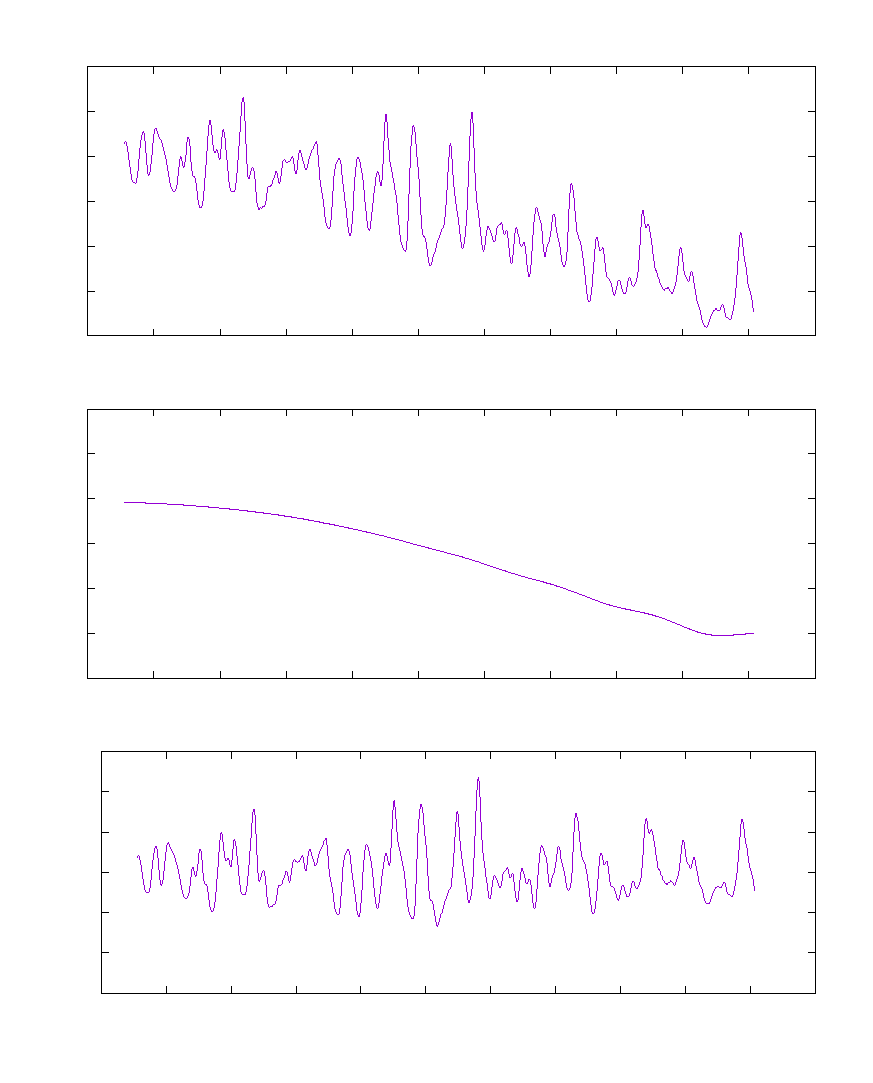
\includegraphics{../images/NO2_conv}}%
    \gplfronttext
  \end{picture}%
\endgroup

  \caption{Absorption cross section of \ch{NO2} in the region around
    \SI{440}{\nano\meter}. From top to bottom there is the complete
    cross section $\sigma$, the broadband part $\sigma^b$ and the
    differential part $\sigma'$. The cross section is adapted to the
    resolution of the spectrograph used in the measurements
    (c.\,f.\ Sec.~\ref{sec:inclusion}).}
  \label{fig:no2-cross}
\end{figure}

As can be seen in Figure~\ref{fig:no2-cross} the
cross sections can be separated into two parts: 

\begin{align*}
  \sigma = \sigma^b + \sigma'.
\end{align*}
One ($\sigma^b$) only weakly wavelength dependent and a narrowband
structure ($\sigma'$) on top which differs strongly for different
species. This narrowband structure is what makes it possible to
distinguish the gases. It is called the \emph{differential adsorption
  bands}. Hence the name of the measurement method. Putting the
results so far into the Lambert-Beer equation leads to

\begin{align*}
  I(\lambda, L) & = I_0(\lambda) \exp \left ( \sum_{i=1}^n L \cdot
                  (\sigma^b_j(\lambda) + \sigma'_j(\lambda))\cdot c_j + L[\epsilon_R +
                  \epsilon_M]\right) \\
                & = I'_0(\lambda) \exp \left( \sum_{i=1}^n L \cdot
                  \sigma'_j(\lambda) \cdot c_j \right),
\end{align*}
where all the broadband structure was collected within $I'_0$. This
makes sense, as the $I_0$ spectrum often will not be free of the Rayleigh
and Mie scattering processes and thus they are already taken into
account. Furthermore residual broadband structure can be handled in
the fitting process by adding a polynomial function. Thus the fit
formula becomes

\begin{align}
  f(\lambda) = - \sum_{i=1}^n c_i \cdot L \cdot \sigma'_i(\lambda) +
  \sum_k a_k \lambda^k \label{eq:doas-fit},
\end{align}
which is fitted to the Optical Density, where the concentrations $c_i$
and the polynomial coefficients $a_k$ are to be determined. The degree
of the polynomial is generally fixed to \num{4}.

One other technical aspect is that it is necessary to adapt the cross
sections to the used spectrometer. Normally the literature values have
a very high resolution and thus depict structure which the used
instrument cannot detect. The effect of this lower resolution is
that narrow emission lines get smeared out. This smearing out is
called \emph{instrument function}. In order to determine it, one can measure the
spectrum of a Mercury lamp and use one of the emission lines as a
convolution kernel. The narrow line is broadened and one can assume
that all other used measurements are broadened by the same amount. So
if the cross sections are convoluted with this mercury line, the lower
resolution will be compensated for. This step has to be done before
the actual fitting and in Equation~\eqref{eq:doas-fit} the convoluted
cross sections have to be used.

This DOAS method is used as measurement method in
Section~\ref{sec:ozone-setup}. 

\subsubsection{The CE-DOAS method}
\label{sec:ce-doas}

Since the absorption coefficents $\epsilon$ are so small, a very long
pathlength $L$ is necessary to see a signal using the DOAS method. One
possibility is to really use a very long geometrical pathlength with
mirrors and telescopes. With this it is possible to obtain pathlengths
between \SI{1}{\kilo\meter} and
\SI{10}{\kilo\meter}~\cite{platt}. These so called
\emph{Longpath-DOAS} instruments have advantages, but also a few
disadvantages; one of them clearly being that they need a lot of space
and in the process they average the concentration of the trace gases
over a large column.

An alternative approach is to increase the lightpath by the use of
optical instruments, i.\,e.\ mirrors. Using two highly reflective
mirrors one can obtain very large optical pathlengths, while still
having a managable geometrical pathlength. The price to pay by
taking this approach is that the light pathlength becomes
wavelength dependent due to the nature of highly reflective mirrors.

In this paragraph, I will generalize the DOAS approach keeping in mind
that the pathlength is not constant anymore. On the way I will try to
separate two effects on the pathlength. First the shortening due to
the absorption by the trace gases and secondly the influence by the
reflectivity.

The geometrical setup is the following:

\begin{figure}[htbp]
  \centering
  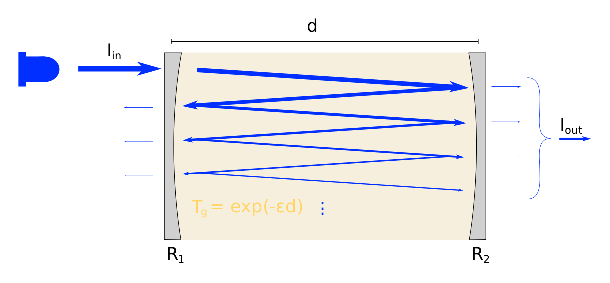
\includegraphics[]{reflection.eps}
  \caption{Geometrical setup of the cavity.}
  \label{fig:cavity}
\end{figure}
where there are two mirrors with reflectivity $R_i$, transmittance $T_i$
and absorption $A_i$. They are connected via

\begin{align*}
  R_i + T_i + A_i = 1 \quad i \in{1,2}.
\end{align*}

Additionally, there is the transmittance $T_g$ of the gas in the
cavity. For this the Lambert-Beer law gives

\begin{align*}
  T_g = \exp(-\epsilon d),
\end{align*}
where $d$ is the length of the cavity. Let $I_{\text{in}}$ be some
intensity entering the cavity, then the outgoing intensity
$I_{\text{out}}$ can be computed using a geometric series

\begin{align}
  I_{\text{out}} & = I_{\text{in}} T_1 T_2 T_g \sum_{n=0}^\infty R_1^n R_2^n T_g^{2n}\nonumber\\
  & = I_{\text{in}} T_1 T_2 T_g \cdot \frac{1}{1 - R_1R_2T_g^2},\label{eq:geometric}
\end{align}
where for the last equation $|R_1R_2T_g^2| < 1$ was assumed to hold,
which is clearly true since all entering variables lie between 0 and
1.

With this formula one can compute the sample air intensity $I$
as well as the \emph{zero air} (i.\,e.\ the trace gas free) intensity $I_0$
depending on the different reflectivities and transmittances. In order to do
this there are a few approximations necessary, which are listed in the
following

\begin{enumerate}
\item $I_{\text{in}}$ is the same for both $I$ and $I_0$. This means
  any fluctuations in the light source intensity coming from
  temperature instabilities or other optomechanic effects are
  neglected.
\item I assume $R_1 \approx R_2 \eqqcolon R \approx 1$, meaning $(R -
  1) \ll 1$. Since highly reflective mirrors are used this assumption
  seems reasonable.
\item I assume $\epsilon \cdot d \ll 1$ for both sample and zero
  air. Furthermore I assume that $T_{g,0}/T_{g}$ is negligible. This
  seems reasonable, too, as the absorption in 
  air is comparativly weak and the geometrical pathlength is in the
  order of magnitude of \SI{1}{\meter}.
\item I assume $(R - 1) + \epsilon d \ll 1$, too. This is only a
  slightly stronger condition than the above mentioned two.
\item I assume to be allowed to neglect higher order monomials of the
  form $(R-1)^i(\epsilon d)^j$  with $i+j \geq 2$, $i,j \in \N_0$.
\end{enumerate}

In the following I will always refer to the number of the above
mentioned assumptions, when used. The approximations carried out below
are described in~\cite{platt2009} and~\cite{fiedler2003}.

In this setup the information of the trace gas concentration should
still be obtainable by comparing $I$ and $I_0$. Again an exponential
relation between the two is suspected so the \emph{Cavity Enhanced
  Optical Density} $D_{\text{CE}}$ is introduced via

\begin{align}
  I(\lambda) = I_0(\lambda) \cdot \exp(- D_{\text{CE}}) = I_0(\lambda)
  \cdot \exp(-\delta(\lambda) \cdot L_{\text{eff}}(\lambda)),\label{eq:opt-dens}
\end{align}
where $\delta \coloneqq \epsilon - \epsilon_0$ is the difference
between the absorption coefficients of sample and zero air, i.\,e.\ the
absorption coefficient of the trace gases, and $L_{\text{eff}}$ is the
wavelength dependent \emph{effective pathlength} of the system. Next,
Equation~\eqref{eq:geometric} is plugged into Equation~\eqref{eq:opt-dens}

\begin{align}
  D_{\text{CE}}(\lambda) & \coloneqq \ln\left(
                           \frac{I_0(\lambda)}{I(\lambda)}\right)\nonumber\\
                         & = \ln\left ( \frac{I_{\text{in}}T_1T_2T_{g,0}(1 -
                           (RT_{g,0})^2)^{-1}}{I_{\text{in}}T_1T_2T_g(1 -
                           (RT_g)^2)^{-1}}\right)\nonumber\\
                         & \stackrel{3.}{\approx} \ln\left( \frac{1 -
                           (RT_g)^2}{1 - (RT_{g,0})^2}\right)\label{eq:d_ce},
\end{align}
where the wavelength dependencies were dropped after the first
equation to preserve clarity. In order to evaluate this expression further, a
first investigation of the expression $(RT)^2$ seems reasonable:

\begin{align}
  [RT]^2 & = [R \exp(-\epsilon d)]^2 \nonumber\\
         & \stackrel{3.}{\approx} [R \cdot(1 - \epsilon d)]^2 \nonumber\\
         & = [(1 + (R - 1))\cdot (1 - \epsilon d)]^2 \nonumber\\
         & \stackrel{5.}{\approx} [1 - (1 - R + \epsilon d)]^2 \nonumber\\
         & \stackrel{4.}{\approx} 1 - 2 \cdot (1 - R + \epsilon d)\label{eq:rt}.
\end{align}
Inserting Equation~\eqref{eq:rt} into Equation~\eqref{eq:d_ce} leads to

\begin{align}
  D_{\text{CE}} & \approx \ln \left ( \frac{1 - (1 - 2\cdot ( 1- R +
  \epsilon d))}{1 - (1 - 2 \cdot (1 - R + \epsilon_0 d))}\right)\\
  & = \ln \left ( \frac{1 - R + \epsilon d}{1 - R + \epsilon_0
    d}\right) \\
  & = \ln \left ( 1 + \frac{ \delta d}{1 - R + \epsilon_0 d}\right) \quad
    \text{with } \delta \coloneqq \epsilon - \epsilon_0.
\end{align}
This last equation can be reformulated to

\begin{align}
  \exp(D_{\text{CE}}(\lambda)) - 1 = \frac{I_0(\lambda)}{I(\lambda)} -
  1 = \frac{d}{1 - R(\lambda) + \epsilon_0(\lambda) d} \cdot
  \delta(\lambda)\label{eq:i-1}, 
\end{align}

where all the trace gas information is bundled in
$\delta(\lambda)$. Solving Equation~\eqref{eq:i-1} for $\delta$ and
plugging it into Equation~\eqref{eq:opt-dens} one yields
\begin{align}
  L_{\text{eff}} = \frac{D_{\text{CE}}}{\exp(D_{\text{CE}}) - 1} \cdot
  \underbrace{\frac{d}{1 - R + d\epsilon_0}}_{\eqqcolon L_0}.
\end{align}
With this definition, $L_0$ is completely independent of any
trace gas influences and hence all the trace gas dependence is
restricted to the first term. Furthermore, $L_0$ directly depends on
the mirror reflectivity. All in all, $L_0$ depends only on the geometry
of the setup (if one assumes $\epsilon_0$ to be fixed) and the desired
separation of $L_{\text{eff}}$ is reached.

Looking only at the definition of $L_0$ and comparing it to
Equation~\eqref{eq:i-1} leads to

\begin{align}
  \delta \cdot L_0 = \frac{I_0}{I} - 1 \eqqcolon D_{\text{eff}}, \label{eq:ce-central}
\end{align}
where $D_{\text{eff}}$ is calle \emph{Effective Optical Density}.This
is the central equation for the CE-DOAS evaluation. $I$ and $I_0$ are
measured and $L_0$ only depends on the geometry, so the only place, where
the trace gas concentrations enter into the equation is via $\delta$, which makes
it very easy to fit the concentrations.

In addition, this equation also allows for the determination of the
pathlength $L_0$. Using Helium as sample air there is a rather large
difference and well known $\delta$, which can then be used to determine
$L_0$.

In the actual evaluation (as in the DOAS evaluation) the fit function

\begin{align*}
  f(\lambda) \coloneqq L_0(\lambda)\cdot\sum_{j=1}^n \sigma_j(\lambda)
  \cdot c_j + \sum_i a_i \lambda^i,
\end{align*}
is used, where the parameters $c_j$ and $a_i$ are fitted to
$D_{\text{eff}}$. This is done using the least square method. The
polynomial is again added to compensate for residual broadband
structure and its degree is fixed to \num{4}.

The CE-DOAS method was used for the measurements in
Sections~\ref{sec:silica} to~\ref{sec:vehicle}. 

%%% Local Variables: 
%%% mode: latex
%%% TeX-master: "../Bachelor"
%%% End: 
